\chapter{相关技术与理论基础}

\section{词向量表示}

词嵌入(Word embedding)是文档词汇最流行的表示形式之一,它是特定单词的向量表示,它能够捕获文档中单词的上下文,语义和句法相似性,与其他单词的关系等。
Word2Vec是使用浅层神经网络学习单词嵌入的最流行技术之一,它是由Tomas Mikolov于2013年在Google上提出的。
Word2Vec是一个浅层的两层神经网络,经过训练可以重建单词的上下文语义。 它的输入来源是一个大的单词语料库,通常产生一个具有几百个维度的向量空间,
该语料库中的每个唯一单词都在该空间中分配了一个相应的向量。 词向量位于向量空间中,以便在语料库中共享公共上下文的词在空间中彼此紧邻。 

  Word2Vec是具有单个隐藏层的简单神经网络,并且像所有神经网络一样,它具有权重,并且在训练过程中,其目标是调整这些权重以减少损失函数。 
  但是,Word2Vec不是用于他训练时处理的任务,相反,我们将仅使用其隐藏的权重,将其用作词嵌入,然后将模型的其余部分扔掉。
  这个trick在无监督的特征学习中也有用到,其中训练了自编码器以在隐藏层中压缩输入向量,然后将其解压缩回输出层中的原始向量,
  训练完成后,剥离输出层,仅使用隐藏层,因为它学习了良好的编码功能。
  如果不同的单词在上下文中相似,那么当这些单词作为输入传递时,Word2Vec应该具有相似的输出,
  并且为了具有相似的输出,这些单词在隐藏层中计算出的单词矢量必须相似,因此Word2Vec的动机是为相似上下文中的单词学习相似的单词向量。
Word2Vec能够捕获单词之间的多个不同程度的相似度,从而可以使用词向量来表示语义和句法模式。
可以通过对这些单词的词向量进行代数运算来生成诸如“男人之于女人等于兄弟之于姐妹”的模式,
从而使“兄弟”-“男人” +“女人”的词向量与“姐妹”的词向量表示十分接近,如图\ref{fig:linear-relationships}所示。


\begin{figure}[htbp]
  \centering
  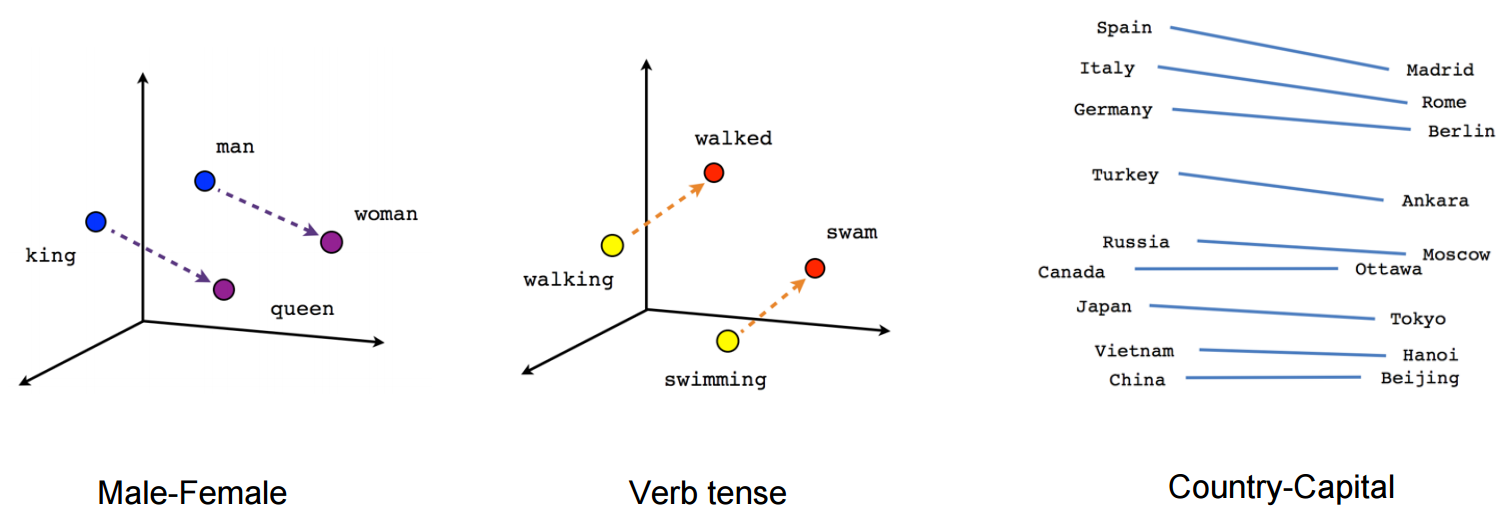
\includegraphics[scale=0.5]{./images/linear-relationships.jpg}
  \caption{词向量之间关系}
  \label{fig:linear-relationships}
\end{figure}


  Word2Vec是一种从原始文本中学习单词嵌入的计算效率特别高的预测模型,
它主要有两种方式,连续词袋(CBOW)模型和Skip-Gram模型,如图\ref{fig:word2vec_diagrams}。
\begin{figure}[htbp]
  \centering
  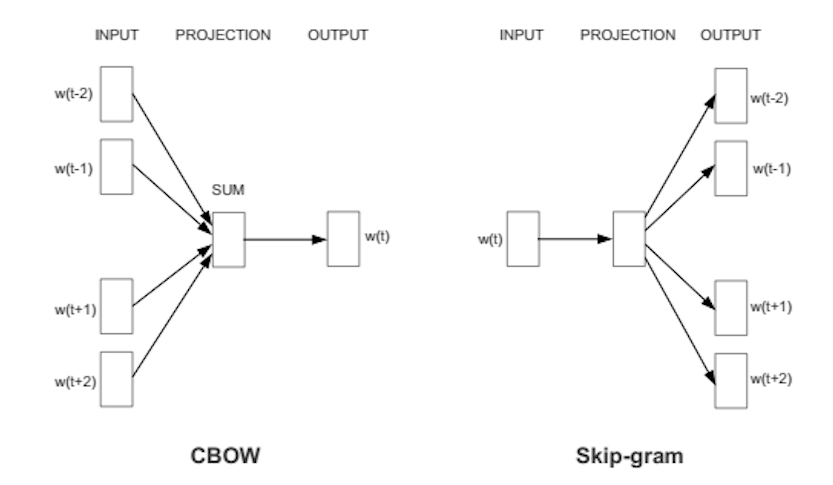
\includegraphics[scale=0.5]{./images/word2vec_diagrams.png}
  \caption{word2vec两种训练方式}
  \label{fig:word2vec_diagrams}
\end{figure}
CBOW模型:此方法将每个单词的上下文作为输入,并尝试预测与上下文相对应的单词。
如图\ref{fig:CBOW}的模型采用C个上下文词,输入是他们的onehot表示,乘以共享矩阵W(维度是V*N)求均值
得到的结果作为隐藏层,是一个N维的矩阵,隐藏层向量乘以输出权重矩阵W'得到输出向量,即为从上下文
中扣出的单词。


\begin{figure}[htbp]
  \centering
  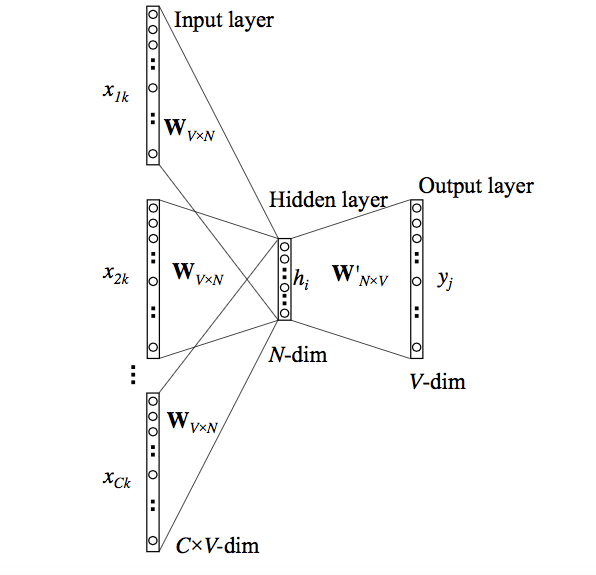
\includegraphics[scale=0.4]{./images/CBOW.jpg}
  \caption{CBOW}
  \label{fig:CBOW}
\end{figure}


给定一个单词,Skip-gram模型的伪造任务是尝试预测其相邻单词,可以简单的看作将cbow模型反过来。

\begin{figure}[htbp]
  \centering
  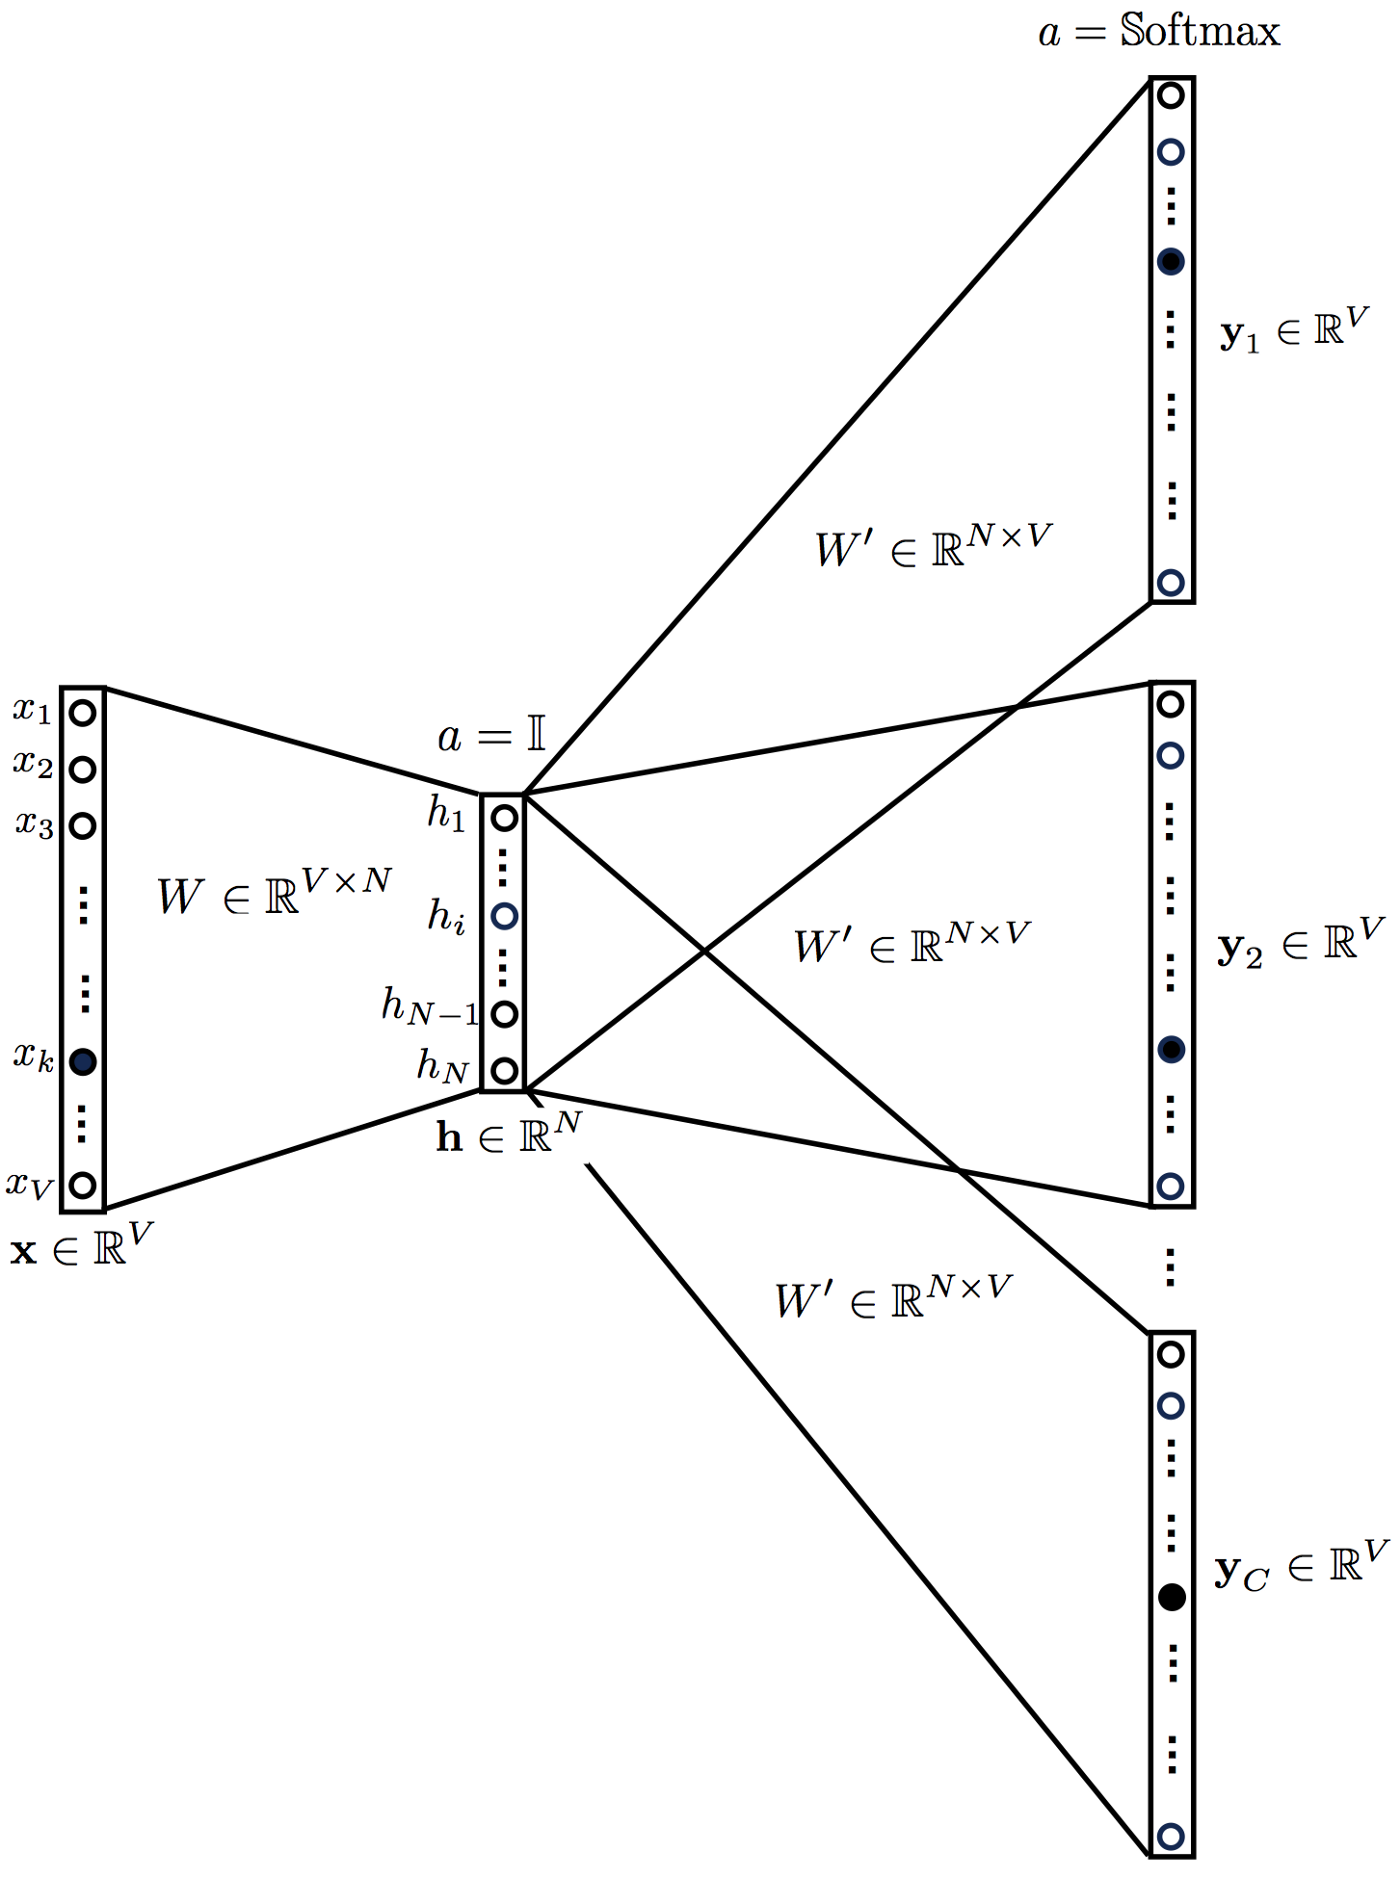
\includegraphics[scale=0.15]{./images/skip.jpg}
  \caption{skip-gram}
  \label{fig:skip}
\end{figure}

\section{预训练模型}

\subsection{RNN}

循环神经网络(RNN)是一种神经网络,其中前一步的输出将作为输入输入到当前步骤。在传统的神经网络中,
所有输入和输出都是彼此独立的,但是在例如需要预测句子的下一个单词的情况下,需要前一个单词,
因此需要记住前一个单词。因此,RNN诞生了,它借助“隐藏层”解决了这个问题。
RNN的主要和最重要的功能是“隐藏状态”,它可以记住一些有关序列的信息。

RNN有一个“内存”,可以记住有关已计算内容的所有信息。它对每个输入使用相同的参数,
因为它在所有输入或隐藏层上执行相同的任务以产生输出,与其他神经网络不同,这降低了参数的复杂性。
RNN通过为所有层提供相同的权重和偏差将独立激活转换为相关激活,
从而通过将每个输出作为下一个隐藏层的输入来降低增加参数的复杂性并存储每个先前的输出。

\begin{figure}[htbp]
  \centering
  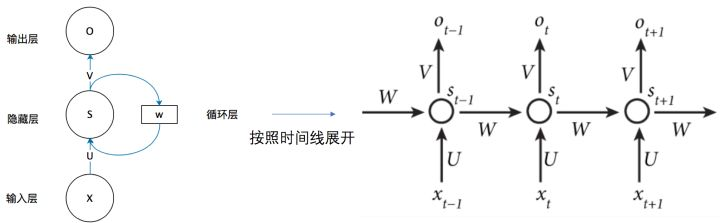
\includegraphics[scale=0.5]{./images/rnn.jpg}
  \caption{RNN}
  \label{fig:rnn}
\end{figure}

上图\ref{fig:rnn}显示了将RNN 展开为完整的网络,rnn可以被我们展开为我们想要的任意层数。例如,
如果我们关心的序列是5个单词的句子,则该网络将展开为5层神经网络,每个单词一层。对于上图具体来说,
$x_{t}$是时刻t的输入,例如,$x_{1}$ 可以是与句子的第二个单词相对应的one-hot向量。
$s_{t}$是时刻t的隐藏状态,这是网络的“记忆”,$s_{t}$根据先前的隐藏状态和当前步骤的输入来计算

\begin{equation}
  s_{t}=f\left(U x_{t}+W s_{t-1}\right)
  \end{equation}

该函数f通常是诸如tanh或ReLU之类的非线性函数,$s_{-1}$计算第一个隐藏状态所需的,通常初始化为全零。
$o_{t}$是时刻t的输出,例如,如果我们想预测句子中的下一个单词,那么它将是整个词汇表中概率的向量。o_t = \ mathrm {softmax}(Vs_t)。
